\documentclass[12pt, letterpaper]{article}
\usepackage{graphicx} % Required for inserting images
\usepackage{hyperref}
\usepackage{listings}
\usepackage{amssymb}
\usepackage{amsmath}
\usepackage[english]{babel}
\usepackage{nicefrac, xfrac}
\usepackage{mathtools}
\newcommand{\acc}{\\\hphantom{}\\}
\usepackage[table,xcdraw]{xcolor}
\definecolor{light-gray}{gray}{0.95}
\newcommand{\code}[1]{\colorbox{light-gray}{\texttt{#1}}}
\usepackage[paper=a4paper,left=20mm,right=20mm,bottom=25mm,top=25mm]{geometry}
\renewcommand{\labelenumii}{\arabic{enumi}.\arabic{enumii}}
    \renewcommand{\labelenumiii}{\arabic{enumi}.\arabic{enumii}.\arabic{enumiii}}
    \renewcommand{\labelenumiv}{\arabic{enumi}.\arabic{enumii}.\arabic{enumiii}.\arabic{enumiv}}
\title{Ristrutturazione Officine 1 }
% \author{ Giacomo Biribicchi \and Marco Casu \and Christian Di Manno \and Alessandro Gautieri }
\date{}


\begin{document}

\maketitle

\section{Tipi di Dato}
\subsection{Domini}
\begin{itemize}
    \item create domain $Intger>0$ as integer
    default 0
    check $(value>=0);$
\end{itemize}
\subsection{Tipi}

\section{Vincoli Esterni Ristrutturazione}
\begin{itemize}
    \item Se un dipendente che è una persona dirige un'officina, allora deve lavorarci da almeno 5 anni \acc
    $\forall p,dp,o,a$ $Persona(p) \land Officina(o) \land PersonaDipendente(dp,p)\land AnniAfferenza(dp,a)$ \acc $\land Dirige(dp,o) \rightarrow a>5 \land Lavora(o,dp)$
    \item Clienti e dipendenti sono separati, un dipendente non può essere cliente e vicecersa \acc
    $\lnot \exists c, d, v Cliente(c) \land Dipendente(d) \land cf(s, v) \land cf(d, v)$
\end{itemize} \newpage
\section{UML}
\begin{center}
    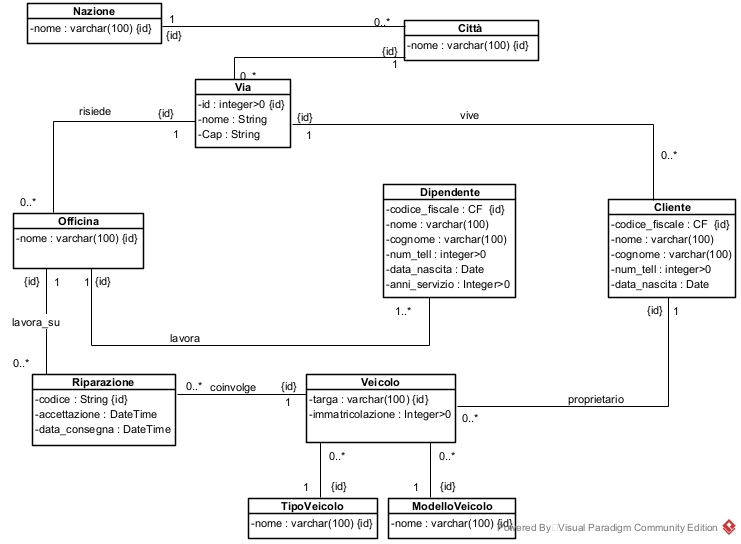
\includegraphics[width=\textwidth]{UML.jpg}
\end{center}


\end{document}

